% Drawing 67/02-1 -- folder 67, batch 02, archive page 33 (PDF page 34).
% Transcription: en bas à droite, un croquis : une sphère, $z$ au pôle nord, $z'$ au pôle sud, quelques méridiens et un point marqué $x$
% Kind: sphere with poles and meridians. Method 2 (schematic redraw from the facsimile). Status: partial.
% Notes: Sphere with z at the north pole and z' at the south pole, three meridians and an equatorial curve. The page carries more overinked strokes on the left (hatching-like) than are drawn; the point x of the transcription is not located with certainty and is placed at the crossing on the left.
% Coordinates: 1 unit = 1 mm = 1/100 of the crop width (bbox in page fractions: [0.76, 0.76, 0.94, 0.88]).
% Redrawn by Claude (claude-opus-5-5), issue #73, 2026-11-07; not checked by a human; not compiled (no TeX in the session).
% Rights: reproduces part of the work -- behind RENDER_TRANSCRIPTS, never published by itself.
\documentclass[tikz,border=3pt]{standalone}
\usepackage{amsmath,amssymb}
\usetikzlibrary{patterns,arrows.meta}
\tikzset{pencil/.style={black!45}, struck/.style={black!35}, mark/.style={circle,draw,inner sep=1.3pt}, pt/.style={circle,fill,inner sep=0.9pt}, opt/.style={circle,draw,fill=white,inner sep=1.1pt}}
\begin{document}
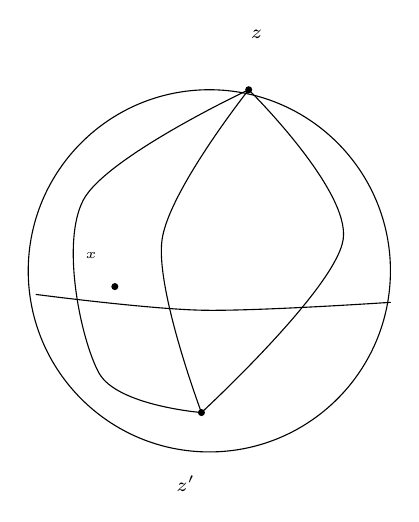
\begin{tikzpicture}[x=1mm,y=1mm,line cap=round,line join=round,font=\scriptsize]
\draw (51,-39) circle[radius=23];
\node[pt] at (56,-16) {};
\node[pt] at (50,-57) {};
\draw plot[smooth, tension=0.55] coordinates {(56,-16) (35,-30) (37,-52) (50,-57)};
\draw plot[smooth, tension=0.55] coordinates {(56,-16) (45,-35) (50,-57)};
\draw plot[smooth, tension=0.55] coordinates {(56,-16) (68,-35) (50,-57)};
\draw plot[smooth, tension=0.55] coordinates {(29,-42) (50,-44) (74,-43)};
\node[pt] at (39,-41) {};
\node[inner sep=1pt] at (36,-37) {\tiny $x$};
\node[inner sep=1pt] at (57,-9) {\scriptsize $z$};
\node[inner sep=1pt] at (48,-66) {\scriptsize $z'$};
\end{tikzpicture}
\end{document}
